%% ---------------------------------------------------------------------------
%% WireGuard-Verified -- technical report.
%%
%% Formatted after the IEEE Symposium on Security and Privacy (Oakland) house
%% style: US Letter, two columns, 10pt Times, IEEEtran conference class, and
%% arabic section numbering with left-aligned bold headings.
%%
%% Build:  make report            (or: latexmk -pdf main.tex, with TEXINPUTS
%%                                 pointing at ./vendor)
%%
%% The class itself is vendored under vendor/ -- see vendor/README.md for why.
%%
%% NOTHING NUMERIC IS TYPED IN THIS DOCUMENT.  Every table and figure under
%% generated/ is produced by scripts/render_tables.py and tools/figures.py, and
%% every quantity the prose states is a macro defined in generated/facts.tex,
%% which those scripts derive from results/results.json, tools/wire.py,
%% tools/pqcost.py, expectations.yaml and the Makefile.  If a number here has
%% no macro behind it, that is a bug: see scripts/render_tables.py.
%% ---------------------------------------------------------------------------
\documentclass[conference,letterpaper,10pt]{IEEEtran}

\usepackage[T1]{fontenc}
\usepackage[utf8]{inputenc}
\usepackage{booktabs}
\usepackage{amsmath,amssymb}
\usepackage{tikz}
\usepackage{xcolor}
\usepackage{microtype}
\usepackage{url}
\usepackage[hidelinks]{hyperref}
\usepackage{cite}

%% --- IEEE S&P sectioning ---------------------------------------------------
%% IEEEtran numbers sections with centred roman numerals.  S&P uses arabic
%% numbers with a trailing period and left-aligned bold headings, so both the
%% counters and the heading format are redefined here.  Subsubsections are
%% run-in, which is also the S&P look and which keeps the document from
%% acquiring a fourth level of hierarchy it does not need.
%%
%% Two families of macro have to change, which is easy to get half-right:
%% \thesection is what \ref and the table of contents show, while
%% \thesectiondis is what IEEEtran prints in the heading itself.  Redefining
%% only the first gives arabic cross-references above roman headings.
\renewcommand{\thesection}{\arabic{section}}
\renewcommand{\thesubsection}{\thesection.\arabic{subsection}}
\renewcommand{\thesubsubsection}{\thesubsection.\arabic{subsubsection}}

\makeatletter
\def\thesectiondis{\thesection.}
\def\thesubsectiondis{\thesubsection.}
\def\thesubsubsectiondis{\thesubsubsection.}

\renewcommand\section{\@startsection{section}{1}{\z@}%
  {2.4ex \@plus 1ex \@minus .2ex}{1.2ex \@plus .2ex}%
  {\normalfont\large\bfseries}}
\renewcommand\subsection{\@startsection{subsection}{2}{\z@}%
  {2.0ex \@plus 1ex \@minus .2ex}{0.8ex \@plus .2ex}%
  {\normalfont\normalsize\bfseries}}
\renewcommand\subsubsection{\@startsection{subsubsection}{3}{\z@}%
  {1.4ex \@plus 1ex \@minus .2ex}{-0.6em}%
  {\normalfont\normalsize\bfseries}}
\makeatother

%% --- Local conventions -----------------------------------------------------
\definecolor{okgreen}{HTML}{2F6F4E}
\definecolor{badred}{HTML}{A33A2A}

%% Outcome markers used by the generated results table.  Defined here so the
%% generator emits semantic commands rather than presentation.
\newcommand{\ok}{\textcolor{okgreen}{\textbf{proved}}}
\newcommand{\attack}{\textcolor{badred}{\textbf{attack found}}}
\newcommand{\inconcl}{\textcolor{black!60}{inconclusive}}
\newcommand{\nonterm}{\textcolor{black!60}{non-terminating}}

%% Bold run-in lead for a paragraph.  The report uses these in place of a
%% third and fourth level of section numbering: a reader scanning a column
%% should be able to see what each paragraph is for without a heading for
%% every one of them.
\newcommand{\para}[1]{\par\smallskip\noindent\textbf{#1}\space}

%% Every quantity the prose quotes.  Generated; see the header comment above.
%% -----------------------------------------------------------------
%% GENERATED by scripts/render_tables.py -- do not edit.
%%
%% Every quantity the report's prose states is defined here, from
%% results/results.json, tools/wire.py, tools/pqcost.py,
%% expectations.yaml or the Makefile.  A number with no macro is a
%% number the report is not entitled to state.
%% -----------------------------------------------------------------

%% --- outcomes, counted over properties (one per table row) -------
\newcommand{\wgProps}{18}
\newcommand{\wgVerdicts}{23}
\newcommand{\wgProved}{11}
\newcommand{\wgAttacks}{3}
\newcommand{\wgInconcl}{1}
\newcommand{\wgNonterm}{3}
\newcommand{\wgPvProps}{12}
\newcommand{\wgPvProved}{6}
\newcommand{\wgPvNonterm}{3}
\newcommand{\wgTamProps}{6}
\newcommand{\wgTamProved}{5}
\newcommand{\wgTamNonterm}{0}
\newcommand{\wgExpectations}{18}

%% --- cost --------------------------------------------------------
\newcommand{\wgBudget}{300}
\newcommand{\wgMemCap}{2.8}
\newcommand{\wgPvSpan}{\textit{n/r}}
\newcommand{\wgTamSpan}{\textit{n/r}}
\newcommand{\wgSuiteSeconds}{---}
\newcommand{\wgTamSteps}{7--18}

%% --- verifiers ---------------------------------------------------
\newcommand{\wgProVerif}{ProVerif}
\newcommand{\wgTamarin}{Tamarin~1.12.0}

%% --- wire format -------------------------------------------------
\newcommand{\wgInitBytes}{148}
\newcommand{\wgRespBytes}{92}
\newcommand{\wgFields}{25}
\newcommand{\wgFieldsModelled}{7}
\newcommand{\wgFieldsUnmodelled}{18}

%% --- post-quantum arithmetic --------------------------------------
\newcommand{\wgKemFiveInit}{916}
\newcommand{\wgKemInit}{1300}
\newcommand{\wgKemResp}{1148}
\newcommand{\wgKemTenInit}{1684}
\newcommand{\wgKemGrowth}{8.8}
\newcommand{\wgKemTenGrowth}{11.4}
\newcommand{\wgIpvsixMtu}{1280}
\newcommand{\wgIpvsixPayload}{1232}
\newcommand{\wgOvershoot}{68}
\newcommand{\wgPaths}{5}

%% --- did this run record per-query wall-clock cost? ---------------
%% False when results/ predates cost recording; the report then omits
%% the cost figure rather than showing an empty one.
\newif\ifwgtimings
\wgtimingsfalse


\begin{document}

\title{Symbolic Verification of the WireGuard Handshake\\
and Its Post-Quantum Migration Cost}

\author{\IEEEauthorblockN{Qiyue Zhao}}

\maketitle

\begin{abstract}
We present a verification artifact for the WireGuard handshake in which a
single protocol transcription drives two symbolic provers and every number
printed in this paper is generated from what those provers wrote. The design
buys two things at once: any difference between the verdicts is attributable
to the prover rather than to the modelling, and no claim in the text can
outlive the run that produced it.

Four results follow. \emph{Firstly}, a controlled pair of models isolates what
the pre-shared key of \texttt{IKpsk2} contributes: against an attacker granted
a discrete-logarithm oracle after the session closes, transport-key secrecy is
proved when the pre-shared key is secret and refuted when it is published,
with the models otherwise identical. \emph{Secondly}, key-compromise
impersonation resistance is located rather than asserted---with the
responder's static key leaked the responder does commit transport keys to a
session it attributes to an honest peer, and never accepts traffic on it; the
static-ephemeral term \(se\) holds that interval open. \emph{Moreover}, an
arithmetic analysis carries post-quantum parameter sizes past the
cryptography and into the network layer, where an in-band ML-KEM-768
initiation reaches \wgKemInit\,B against a usable IPv6 minimum-MTU payload of
\wgIpvsixPayload\,B. \emph{Finally}, the failures are reported alongside the
proofs: \wgNonterm{} queries were left undecided, and they are in the same
table as the rest.

The numbers make the comparison concrete. Across \wgProps{} properties the two
provers return \wgProved{} proofs, \wgAttacks{} attacks, \wgInconcl{}
inconclusive and \wgNonterm{} non-terminating verdicts.
\ifwgtimings
ProVerif decides \the\numexpr\wgPvProps-\wgPvNonterm\relax{} of \wgPvProps{}
properties in \wgPvSpan\,s and exhausts a \wgBudget\,s budget on the other
\wgPvNonterm; Tamarin decides all \wgTamProps, including both
key-compromise-impersonation levels, in \wgTamSpan\,s and \wgTamSteps{}
constraint-solving steps.
\else
ProVerif decides \the\numexpr\wgPvProps-\wgPvNonterm\relax{} of \wgPvProps{}
properties and exhausts a \wgBudget\,s budget on the other \wgPvNonterm;
Tamarin decides all \wgTamProps, including both key-compromise-impersonation
levels, in \wgTamSteps{} constraint-solving steps.
\fi
The in-band initiation grows by a factor of \wgKemGrowth{} at ML-KEM-768 and
overshoots the IPv6 minimum-MTU payload by \wgOvershoot\,B, so no in-band
construction has a guaranteed path---which is why separate-channel designs
are architecturally necessary rather than merely convenient.
\end{abstract}

\section{Introduction}
\label{sec:intro}

WireGuard~\cite{donenfeld2017wireguard} is a VPN protocol whose handshake
instantiates the Noise \texttt{IKpsk2} pattern~\cite{perrin2018noise}. It sits
in the mainline Linux kernel and carries production traffic, so questions
about its security properties, and about what migrating it to post-quantum
primitives would cost, are engineering questions with deployed consequences.

The protocol has been analysed before: symbolically by Donenfeld and
Milner~\cite{donenfeld2018formal}, and in the computational model by Lipp,
Blanchet and Bhargavan~\cite{lipp2019cryptoverif}. This work is an independent
reconstruction from the specification and claims no new vulnerability. Its
contribution lies elsewhere, in two places that prior analyses did not
occupy. The first is methodological: the handshake is transcribed \emph{once}
and handed to two provers, so that a disagreement between them is evidence
about the provers rather than about two people's modelling habits. The second
is that the analysis does not stop at the cryptography. Post-quantum
parameter sizes are followed through to datagram sizes and from there to path
MTUs, which is where the migration cost actually becomes visible.

\begin{figure*}[t]
\centering
\resizebox{\textwidth}{!}{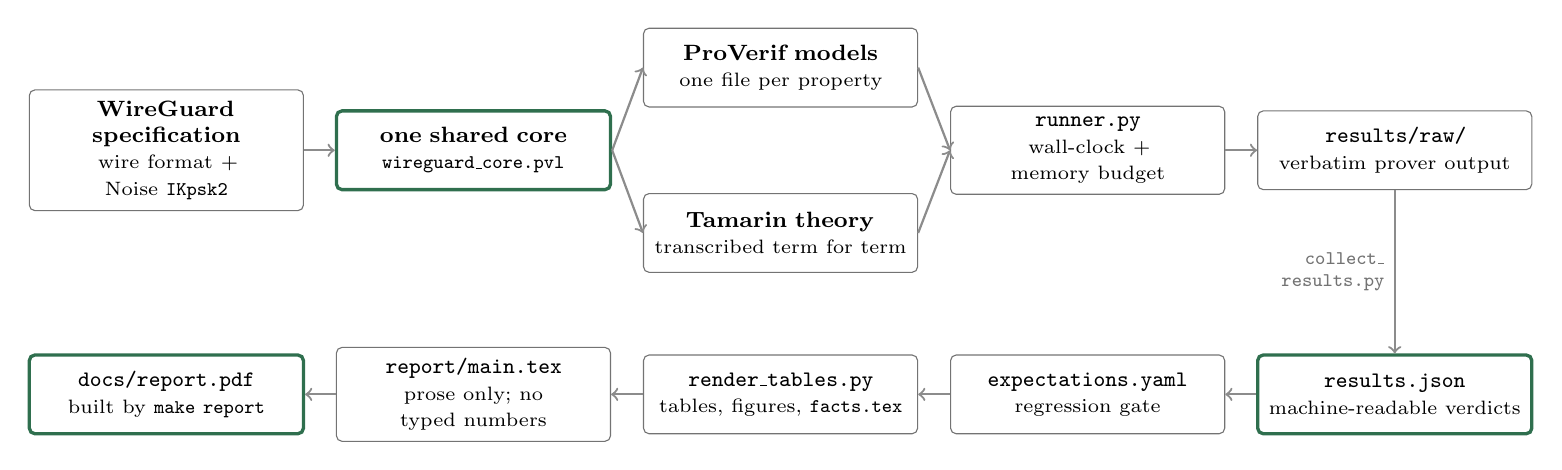
\begin{tikzpicture}[x=1cm,y=1cm,font=\footnotesize,
    bx/.style={draw=black!55,rounded corners=2pt,align=center,inner sep=4pt,
               text width=3.2cm,minimum height=1.0cm},
    hi/.style={bx,draw=okgreen,very thick},
    lnk/.style={->,thick,black!45}]

  \node[bx] (spec) at (1.7,0)
    {\textbf{WireGuard specification}\\{\scriptsize wire format $+$ Noise \texttt{IKpsk2}}};
  \node[hi] (core) at (5.6,0)
    {\textbf{one shared core}\\{\scriptsize \texttt{wireguard\_core.pvl}}};
  \node[bx] (pv) at (9.5,1.05)
    {\textbf{ProVerif models}\\{\scriptsize one file per property}};
  \node[bx] (tam) at (9.5,-1.05)
    {\textbf{Tamarin theory}\\{\scriptsize transcribed term for term}};
  \node[bx] (run) at (13.4,0)
    {\textbf{\texttt{runner.py}}\\{\scriptsize wall-clock $+$ memory budget}};
  \node[bx] (raw) at (17.3,0)
    {\textbf{\texttt{results/raw/}}\\{\scriptsize verbatim prover output}};

  \node[hi] (json) at (17.3,-3.1)
    {\textbf{\texttt{results.json}}\\{\scriptsize machine-readable verdicts}};
  \node[bx] (exp) at (13.4,-3.1)
    {\textbf{\texttt{expectations.yaml}}\\{\scriptsize regression gate}};
  \node[bx] (gen) at (9.5,-3.1)
    {\textbf{\texttt{render\_tables.py}}\\{\scriptsize tables, figures, \texttt{facts.tex}}};
  \node[bx] (tex) at (5.6,-3.1)
    {\textbf{\texttt{report/main.tex}}\\{\scriptsize prose only; no typed numbers}};
  \node[hi] (pdf) at (1.7,-3.1)
    {\textbf{\texttt{docs/report.pdf}}\\{\scriptsize built by \texttt{make report}}};

  \draw[lnk] (spec) -- (core);
  \draw[lnk] (core.east) -- (pv.west);
  \draw[lnk] (core.east) -- (tam.west);
  \draw[lnk] (pv.east) -- (run.west);
  \draw[lnk] (tam.east) -- (run.west);
  \draw[lnk] (run) -- (raw);
  \draw[lnk] (raw) -- node[left,black!55,font=\scriptsize,align=right]
    {\texttt{collect\_}\\\texttt{results.py}} (json);
  \draw[lnk] (json) -- (exp);
  \draw[lnk] (exp) -- (gen);
  \draw[lnk] (gen) -- (tex);
  \draw[lnk] (tex) -- (pdf);
\end{tikzpicture}
}
\caption{How one protocol description reaches two provers and one report.
The two shaded stages are the load-bearing ones: a single shared core that
both prover front-ends include, and a single machine-readable result file that
every table, figure and quoted number in this paper is generated from. No
number in this document is typed by hand.}
\label{fig:pipeline}
\end{figure*}

\subsection{Contributions}

\para{A controlled experiment isolating the pre-shared key.} The \texttt{psk}
of \texttt{IKpsk2} is widely described as providing post-quantum protection.
Section~\ref{sec:results} makes that claim testable with a pair of models
identical in every respect except whether the pre-shared key is secret, run
against an attacker that gains a discrete-logarithm oracle after the session
completes. Transport-key secrecy is proved in one and refuted in the other.
Because the models differ in exactly one variable, so does the explanation.

\para{Locating key-compromise impersonation resistance.} With the responder's
own static key in the attacker's hands, we show that the responder \emph{does}
commit transport keys for a session it attributes to an honest initiator, and
\emph{never} accepts traffic on that session. Forging message~1 needs only
Diffie-Hellman terms computable from the leaked scalar; deriving the transport
keys additionally needs the static-ephemeral term \(se=\mathrm{DH}(e_r,S_i)\),
which does not follow. The property therefore lives in the interval between
committing key material and accepting traffic---a distinction a single
monolithic ``session established'' event would hide entirely.

\para{A three-dimensional account of post-quantum migration cost.}
Section~\ref{sec:pq} follows a chain of consequences: KEM parameter sizes
determine datagram sizes, datagram sizes meet path MTUs, and a datagram that
exceeds the IPv6 minimum MTU has no guaranteed path. An in-band ML-KEM-768
initiation is \wgKemInit\,B against a usable payload of \wgIpvsixPayload\,B.
The cost of migration is not only computational: it appears simultaneously in
packet size, in path reachability, and in the strength of the binding
assumption the KEM must satisfy.

\para{Reported failure, and numbers that cannot drift.} Of \wgPvProps{}
ProVerif properties, \wgPvNonterm{} did not terminate within the budget this
project set itself, and two of them were decided by Tamarin in seconds. Both facts are in the result
table alongside the proofs. So is the mechanism that keeps them honest: the
tables, the figures and every quantity quoted in this text are generated from
\texttt{results/results.json} at build time (Figure~\ref{fig:pipeline}), so a
sentence in this paper cannot survive a run that contradicts it.

\subsection{Scope}

This paper concerns the handshake. The data plane, the cookie-based
rate-limiting mechanism, and endpoint roaming are network-layer behaviours
with no counterpart in an abstract Noise model;
Section~\ref{sec:modelling} states for each wire-format field whether it is
represented in the models and, where it is not, why. Reproduction
instructions and the resource profile of every result accompany the artifact.

\section{Background and Related Work}
\label{sec:background}

\subsection{What the WireGuard handshake computes}

WireGuard's handshake is Noise \texttt{IKpsk2}, instantiated with X25519,
ChaCha20-Poly1305 and BLAKE2s. The initiator knows the
responder's static public value in advance---this is what makes the pattern
\texttt{IK} rather than \texttt{XX}---and the exchange completes in two
messages, an initiation of \wgInitBytes\,B and a response of \wgRespBytes\,B
(Figure~\ref{fig:flow}).

\begin{figure}[t]
\centering
\resizebox{\columnwidth}{!}{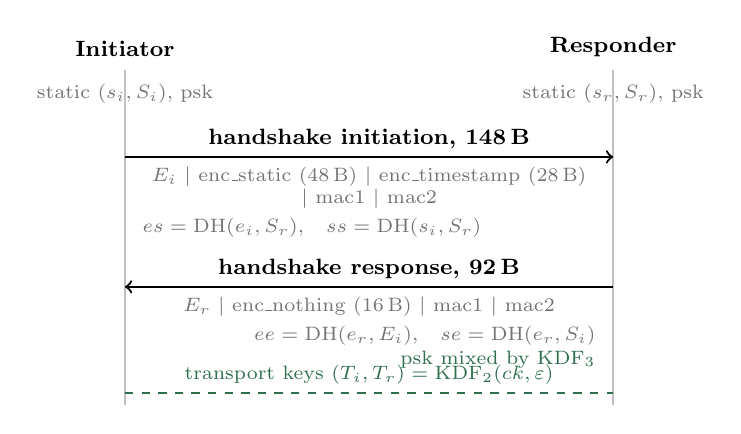
\begin{tikzpicture}[x=1cm,y=1cm,font=\footnotesize]
  \draw[black!25,thick] (0,-0.25) -- (0,-4.5);
  \draw[black!25,thick] (6.2,-0.25) -- (6.2,-4.5);
  \node[anchor=south] at (0,-0.2) {\bfseries Initiator};
  \node[anchor=south] at (6.2,-0.2) {\bfseries Responder};
  \node[anchor=north,black!55,font=\scriptsize] at (0,-0.3)
    {static $(s_i,S_i)$, psk};
  \node[anchor=north,black!55,font=\scriptsize] at (6.2,-0.3)
    {static $(s_r,S_r)$, psk};

  \draw[->,thick] (0,-1.35) -- (6.2,-1.35);
  \node[anchor=south,inner sep=2pt] at (3.1,-1.32)
    {\bfseries handshake initiation, 148\,B};
  \node[anchor=north,black!55,font=\scriptsize,align=center,inner sep=2pt]
    at (3.1,-1.4)
    {$E_i$ $\mid$ enc\_static (48\,B) $\mid$ enc\_timestamp (28\,B)\\
      $\mid$ mac1 $\mid$ mac2};
  \node[anchor=west,black!55,font=\scriptsize] at (0.1,-2.25)
    {$es=\mathrm{DH}(e_i,S_r)$,\quad $ss=\mathrm{DH}(s_i,S_r)$};

  \draw[<-,thick] (0,-3.0) -- (6.2,-3.0);
  \node[anchor=south,inner sep=2pt] at (3.1,-2.97)
    {\bfseries handshake response, 92\,B};
  \node[anchor=north,black!55,font=\scriptsize,inner sep=2pt] at (3.1,-3.05)
    {$E_r$ $\mid$ enc\_nothing (16\,B) $\mid$ mac1 $\mid$ mac2};
  \node[anchor=east,black!55,font=\scriptsize] at (6.1,-3.62)
    {$ee=\mathrm{DH}(e_r,E_i)$,\quad $se=\mathrm{DH}(e_r,S_i)$};
  \node[anchor=east,okgreen,font=\scriptsize] at (6.1,-3.92)
    {psk mixed by $\mathrm{KDF}_3$};

  \draw[okgreen,dashed,thick] (0,-4.35) -- (6.2,-4.35);
  \node[anchor=south,okgreen,font=\scriptsize,inner sep=2pt] at (3.1,-4.32)
    {transport keys $(T_i,T_r)=\mathrm{KDF}_2(ck,\varepsilon)$};
\end{tikzpicture}
}
\caption{The two handshake messages, their sizes on the wire, and the
Diffie-Hellman terms each contributes to the key schedule. Sizes are computed
from the field layout of Section~\ref{sec:modelling}, not transcribed.}
\label{fig:flow}
\end{figure}

Four Diffie-Hellman terms enter the key schedule, and every property in this
paper turns on which of them an attacker can compute:

\begin{itemize}\itemsep2pt
\item \(es=\mathrm{DH}(e_i,S_r)\), initiator ephemeral against responder
      static, binding message~1 to its intended recipient;
\item \(ss=\mathrm{DH}(s_i,S_r)\), static-static, which gives \texttt{IK} its
      first-message authentication;
\item \(ee=\mathrm{DH}(e_r,E_i)\), ephemeral-ephemeral, the term that carries
      forward secrecy;
\item \(se=\mathrm{DH}(e_r,S_i)\), responder ephemeral against initiator
      static, which authenticates the initiator to the responder in
      message~2.
\end{itemize}

A pre-shared key, when configured, is mixed in by \(\mathrm{KDF}_3\) during
message~2, yielding a chaining key, a value \(\tau\) folded into the
transcript hash, and an AEAD key. Because \(\tau\) enters the transcript, a
mismatched pre-shared key makes the authenticated decryption in message~2 fail
rather than producing a silently divergent session.

\para{Beyond the Noise pattern.} WireGuard adds a TAI64N timestamp, session
indices, and two MAC fields. The first, \texttt{mac1}, is keyed by a hash of
the recipient's static public value; it demonstrates knowledge of that value
and suppresses unsolicited traffic, but is not a cryptographic authenticator.
The second, \texttt{mac2}, carries a cookie under load. Both are
consequential for the correspondence of Section~\ref{sec:modelling} and for
what the symbolic model can and cannot say.

\subsection{Symbolic verification, and why two provers}

Both tools used here work in the Dolev-Yao model~\cite{dolev1983security}: the
attacker controls the network completely and the cryptographic primitives are
perfect.

\para{ProVerif.} ProVerif~\cite{blanchet2016proverif} translates an applied
pi-calculus process into Horn clauses and saturates them. It is fully
automatic and fast, handles an unbounded number of sessions, and
over-approximates: a proof is sound, while a reported attack may occasionally
be spurious. Saturation either converges or it does not, and when it does not
the tool gives no partial answer.

\para{Tamarin.} Tamarin~\cite{meier2013tamarin} works with multiset rewriting
and constraint solving, represents mutable state directly, and normalises
Diffie-Hellman terms natively. It reasons backwards from the property rather
than forwards from the rules, which turns out to matter for exactly the
queries ProVerif could not settle.

\para{Stating authentication precisely.} Authentication is stated throughout
in Lowe's hierarchy~\cite{lowe1997hierarchy}: aliveness, weak agreement,
non-injective agreement, injective agreement. Naming the level explicitly
matters here, because the key-compromise result of
Section~\ref{sec:results} is precisely a case of two adjacent levels
separating.

\subsection{Related work}

\para{Prior analyses of WireGuard.} Donenfeld and
Milner~\cite{donenfeld2018formal} give a symbolic analysis in Tamarin covering
the handshake and its state machine. Lipp, Blanchet and
Bhargavan~\cite{lipp2019cryptoverif} give a mechanised computational proof in
CryptoVerif, which yields concrete bounds this work cannot. Our contribution
relative to both is not a stronger result on the same property, but the
deliberate pairing of two symbolic tools on one transcription, and the
extension of the analysis past the cryptography into path reachability.

\para{Post-quantum WireGuard.} Hülsing et
al.~\cite{hulsing2021pqwireguard} redesign the handshake around KEMs directly,
and Rosenpass~\cite{rosenpass2023} instead runs a post-quantum key agreement
on a separate channel and injects the result into WireGuard's pre-shared key
slot. Section~\ref{sec:pq} does not propose a third design; it supplies the
arithmetic that explains why the second shape exists.

\para{KEM binding.} Cremers, Dax and Medinger~\cite{cremers2024kembinding}
systematise binding properties for KEMs and provide the vocabulary in which
the result of Section~\ref{sec:results} is stated. The property that separates
our two KEM models is MAL-BIND-K-PK.

\section{How the Models Are Built and Kept Honest}
\label{sec:modelling}

Table~\ref{tab:scope} states what the artifact contains. The figures in it are
counted from the files themselves at build time, so the description cannot
drift away from the thing it describes.

\begin{table}[t]
\centering
\caption{Verification scope, measured from the repository rather than
described. ``Properties'' counts rows of the result matrix
(Table~\ref{tab:results}), not queries: a model file may carry several.}
\label{tab:scope}
\footnotesize
\begin{tabular}{@{}lrrr@{}}
\toprule
Component & Files & Lines & Properties \\
\midrule
Shared ProVerif core (\texttt{lib/}) & 3 & 349 & --- \\
ProVerif query models & 11 & 302 & 12 \\
Tamarin theory & 1 & 236 & 6 \\
Wire-format layout (\texttt{wire.py}) & 1 & 201 & 25 fields \\
\bottomrule
\end{tabular}

\end{table}

\subsection{One transcription, two provers}

The project's central methodological commitment is that any difference between
the two provers' outcomes should be attributable to the provers, not to the
modelling. The handshake is therefore written once, in
\texttt{lib/wireguard\_core.pvl}, and every ProVerif query file includes that
library rather than restating the protocol. The Tamarin model is transcribed
term for term against it, and Section~\ref{sec:discussion} records the two
places where the transcriptions could not be made identical, together with the
reason in each case.

\subsection{Primitives, and one abstraction that decided the project}

\para{Diffie-Hellman with two symbols.} Diffie-Hellman is modelled with two
symbols rather than an iterated exponentiation:
\[
  \mathit{pk}(x), \qquad
  \mathit{dh}(P,y), \qquad
  \mathit{dh}(\mathit{pk}(x),y)=\mathit{dh}(\mathit{pk}(y),x).
\]
Two consequences matter. Because \(\mathit{pk}\) is the only constructor of
the group type, every group element the attacker can supply is \(g^t\) for
some term \(t\) it can build---faithful for a prime-order group, where every
X25519 output is of that form. Because \(\mathit{dh}\) returns key material
rather than a group element, a Diffie-Hellman result cannot re-enter as a
group element, so term depth is bounded by construction.

\para{Why the obvious formulation fails.} This was not a stylistic choice. The
natural formulation \(\mathit{exp}(G,\mathit{exponent}):G\) lets the attacker
build towers \(\mathit{exp}(\mathit{exp}(\mathit{exp}(g,a),b),c)\) that the
single commuting equation does not normalise. With that formulation,
saturation on the secrecy query exhausted the memory budget after roughly
\(1.2\times10^4\) clauses and never terminated; with the two-symbol
formulation the same query is proved well inside the budget
(Table~\ref{tab:results}). The episode is recorded because it decides whether
a symbolic model is usable at all, and it is rarely written down.

\para{A flat transcript hash.} Noise updates \(h \leftarrow
\mathrm{HASH}(h \mathbin\| f)\) after each field. Since \(h\) is never
transmitted and serves only as AEAD associated data, its sole requirement is
that it bind the transcript prefix injectively, so we model \(h\) after step
\(i\) as a distinct collision-resistant function of the entire prefix. Both
formulations bind the same data; the flat one keeps term depth constant. AEAD,
the HKDF chain and the keyed MAC are standard perfect primitives, with one
function symbol per HKDF output position.

\subsection{The attacker, and when it gains each capability}

\begin{figure}[t]
\centering
\resizebox{\columnwidth}{!}{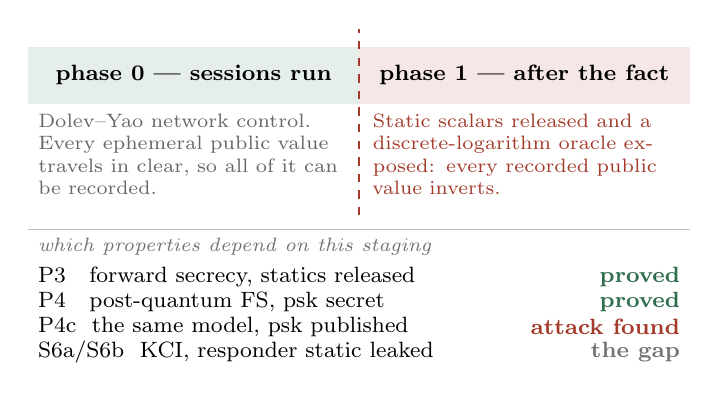
\begin{tikzpicture}[x=1cm,y=1cm,font=\footnotesize]
  \fill[okgreen!12] (0,0) rectangle (4.2,0.72);
  \fill[badred!12]  (4.2,0) rectangle (8.4,0.72);
  \node at (2.1,0.36) {\bfseries phase 0 --- sessions run};
  \node at (6.3,0.36) {\bfseries phase 1 --- after the fact};
  \draw[badred,dashed,thick] (4.2,-1.42) -- (4.2,0.95);

  \node[anchor=north west,text width=3.9cm,black!60,inner sep=2pt,
        font=\scriptsize] at (0.05,-0.06)
    {Dolev--Yao network control. Every ephemeral public value travels in
     clear, so all of it can be recorded.};
  \node[anchor=north west,text width=3.9cm,badred,inner sep=2pt,
        font=\scriptsize] at (4.3,-0.06)
    {Static scalars released and a discrete-logarithm oracle exposed: every
     recorded public value inverts.};

  \draw[black!25] (0,-1.6) -- (8.4,-1.6);
  \node[anchor=west,black!55,font=\scriptsize\itshape] at (0,-1.82)
    {which properties depend on this staging};
  \node[anchor=west] at (0,-2.20) {P3\quad forward secrecy, statics released};
  \node[anchor=east,okgreen] at (8.4,-2.20) {\bfseries proved};
  \node[anchor=west] at (0,-2.52) {P4\quad post-quantum FS, psk secret};
  \node[anchor=east,okgreen] at (8.4,-2.52) {\bfseries proved};
  \node[anchor=west] at (0,-2.84) {P4c\ \ the same model, psk published};
  \node[anchor=east,badred] at (8.4,-2.84) {\bfseries attack found};
  \node[anchor=west] at (0,-3.16) {S6a/S6b\ \ KCI, responder static leaked};
  \node[anchor=east,black!55] at (8.4,-3.16) {\bfseries the gap};
\end{tikzpicture}
}
\caption{Compromise is staged, never built in. Phase~0 is the classical
Dolev-Yao attacker; phase~1 releases the static scalars and a
discrete-logarithm oracle, strictly after every phase-0 session. The
key-compromise queries sit outside this staging, because there the compromise
is part of the scenario rather than a sequel to it.}
\label{fig:compromise}
\end{figure}

The attacker is Dolev-Yao. Compromise is never a built-in capability: each
class of secret is revealed by an explicit action, so every query states which
compromises it tolerates, and a proof cannot silently depend on an assumption
nobody wrote down.

\para{Staging a quantum transition.} Post-quantum capability is expressed with
ProVerif's phase mechanism (Figure~\ref{fig:compromise}). Phase~0 is the
classical attacker. In phase~1 the attacker gains a discrete-logarithm oracle,
private in phase~0 and exposed only by a phase-1 process. Since every
ephemeral public value travels in clear, an attacker that recorded phase-0
traffic can invert all of it once phase~1 begins. This is the standard
formalisation of harvest-now-decrypt-later, and it is what makes post-quantum
forward secrecy a property rather than a slogan.

\para{Compromise as part of the scenario.} Key-compromise impersonation needs
the opposite arrangement: the responder's static key is in the attacker's
hands \emph{while} the session runs, not afterwards. That is an ordering
constraint over individual events rather than a global staging, which is why
those queries are posed to Tamarin with action facts and why the two provers
do not divide this work symmetrically.

\subsection{From wire format to model terms}

A formal model earns its authority from the fidelity of its correspondence to
the artifact it claims to describe. We therefore maintain a field-by-field
mapping from the wire format to terms in the models, and make it
machine-checkable rather than a promise.

\para{Offsets are derived, never written.} \texttt{tools/wire.py} is the
single source of truth for the layout. Offsets are accumulated from the field
lengths, so a corrected length cannot leave a stale offset behind it, and the
computed totals are checked against the specification figures of
\wgInitBytes, \wgRespBytes, 64 and 16\,B. Tables~\ref{tab:wireinit}
and~\ref{tab:wireresp} are rendered from that same structure, which is also
what \texttt{scripts/verify\_wire\_table.py} cross-checks the models against.
Of \wgFields{} fields across the four message types, \wgFieldsModelled{} carry
a model term and \wgFieldsUnmodelled{} deliberately do not.

\begin{table}[t]
\centering
\caption{Handshake initiation, \wgInitBytes\,B. Offsets are derived from
lengths; ``model term'' names the corresponding term in the shared ProVerif
core, and a dash marks a field deliberately outside the models.}
\label{tab:wireinit}
\footnotesize
\begin{tabular}{@{}rrll@{}}
\toprule
Off & Len & Field & Model term \\
\midrule
0 & 1 & \texttt{message\_type} & \textcolor{black!45}{---} \\
1 & 3 & \texttt{reserved} & \textcolor{black!45}{---} \\
4 & 4 & \texttt{sender\_index} & \textcolor{black!45}{---} \\
8 & 32 & \texttt{unencrypted\_ephemeral} & $E_i=\mathit{pk}(e_i)$ \\
40 & 48 & \texttt{encrypted\_static} & $\mathrm{aead}(k_1,0,S_i,h_1)$ \\
88 & 28 & \texttt{encrypted\_timestamp} & $\mathrm{aead}(k_2,0,\mathit{ts},h_2)$ \\
116 & 16 & \texttt{mac1} & $\mathrm{mac}(H(L\|S_r),\cdot)$ \\
132 & 16 & \texttt{mac2} & \textcolor{black!45}{---} \\
\bottomrule
\end{tabular}

\end{table}

\begin{table}[t]
\centering
\caption{Handshake response, \wgRespBytes\,B. Note that \texttt{mac1} here is
keyed by the \emph{initiator's} static public value, which is what makes
identity hiding conditional.}
\label{tab:wireresp}
\footnotesize
\begin{tabular}{@{}rrll@{}}
\toprule
Off & Len & Field & Model term \\
\midrule
0 & 1 & \texttt{message\_type} & \textcolor{black!45}{---} \\
1 & 3 & \texttt{reserved} & \textcolor{black!45}{---} \\
4 & 4 & \texttt{sender\_index} & \textcolor{black!45}{---} \\
8 & 4 & \texttt{receiver\_index} & \textcolor{black!45}{---} \\
12 & 32 & \texttt{unencrypted\_ephemeral} & $E_r=\mathit{pk}(e_r)$ \\
44 & 16 & \texttt{encrypted\_nothing} & $\mathrm{aead}(k_3,0,\varepsilon,h_5)$ \\
60 & 16 & \texttt{mac1} & $\mathrm{mac}(H(L\|S_i),\cdot)$ \\
76 & 16 & \texttt{mac2} & \textcolor{black!45}{---} \\
\bottomrule
\end{tabular}

\end{table}

\para{What is not modelled, and why.} Four field classes are deliberately
absent, and stating the reason for each is part of the correspondence rather
than an apology for it. \emph{Message type and reserved bytes} serve
demultiplexing; the models use distinct channels instead. \emph{Session
indices} are chosen freely by the sender and carry no security burden, but
they are also what makes endpoint roaming possible---a WireGuard engineering
advantage with no counterpart in an abstract Noise model. \emph{\texttt{mac2}
and the cookie mechanism} are load-shedding devices, and the Dolev-Yao
attacker has no notion of computational cost, so a symbolic model cannot
express the property they provide. \emph{The data-plane counter and its
anti-replay window} lie outside the handshake entirely.

\para{An argued property, not a verified one.} The cookie mechanism deserves
the distinction made explicitly. \texttt{mac1} is keyed by
\(\mathrm{HASH}(\mathtt{LABEL\_MAC1} \mathbin\| S_r)\), so an attacker
ignorant of the responder's static public value cannot produce a message that
survives the first check, and cannot force a Diffie-Hellman operation. That is
a genuine property, and it is genuinely outside the model. We argue it here
rather than claim the models establish it.

\para{Conditional identity hiding.} One field deserves separate mention. As
Table~\ref{tab:wireresp} records, the \texttt{mac1} of the \emph{response} is
keyed by the \emph{initiator's} static public value. An observer holding a
candidate public key can therefore test whether a given response is addressed
to its holder. WireGuard's identity hiding is accordingly conditional: it
protects the initiator's identity from an observer who does not already hold
the candidate keys, and not from one who does. The distinction is visible only
because \texttt{mac1} was modelled explicitly rather than abstracted away.

\subsection{Budgets, expectations, and generated numbers}

\para{Every run is bounded.} Every invocation carries an explicit
address-space cap and wall-clock timeout---\wgMemCap\,GB and \wgBudget\,s on a
single core, a budget chosen to match what remains available on an 8\,GB
laptop with an editor open. The cap matters more than its value: without one,
a runaway query consumes the machine and produces a run that is slow,
irreproducible and hostile to anything else running. With one, a query either
finishes within budget or fails deterministically, which is a reportable
outcome.

\para{Verification as a regression suite.}
\texttt{expectations.yaml} declares the expected verdict for each of
\wgExpectations{} queries, and \texttt{make verify} fails on any mismatch.
Outcomes that are attacks are expectations too: the control model of
Section~\ref{sec:results} is \emph{supposed} to be refuted, and a run in which
it succeeded would indicate that the model had drifted, not that the protocol
had improved.

\para{No number in this paper is typed.} Result tables, figures and every
quantity this text quotes are rendered from \texttt{results/results.json},
\texttt{tools/wire.py} and \texttt{tools/pqcost.py} when the document is
built. An earlier revision of this report was internally consistent and
externally wrong---the tables were generated and correct while the prose
quoted timings from a run nobody could identify. Generating the tables was not
enough, because prose is not data; the numbers in the sentences are now macros
too.

\section{Verification Results}
\label{sec:results}

Table~\ref{tab:results} is the complete result matrix, rendered from
\texttt{results/results.json}. Every cell is populated: proved, refuted,
inconclusive, or non-terminating with a recorded cause and the budget it
consumed. Of \wgProps{} properties, \wgProved{} are proved, \wgAttacks{} are
refuted, \wgInconcl{} is inconclusive and \wgNonterm{} did not terminate.

\begin{table*}[t]
\centering
\caption{Verification outcomes, the complete matrix. \wgProVerif{} and
\wgTamarin, single core, \wgMemCap\,GB address-space cap, \wgBudget\,s
wall-clock budget. \(\dagger\) marks a budget consumed without reaching a
verdict, which is not a time-to-verdict and must not be read as one; \emph{n/r}
marks a run that predates per-query cost recording. Every cell is rendered
from \texttt{results/results.json}.}
\label{tab:results}
\footnotesize
\begin{tabular}{@{}lllrl@{}}
\toprule
ID & Property & Prover & Cost & Outcome \\
\midrule
P1 & Session-key secrecy & ProVerif & \textit{n/r} & \ok \\
P3 & Forward secrecy & ProVerif & \textit{n/r} & \ok \\
P4 & Post-quantum forward secrecy (psk) & ProVerif & \textit{n/r} & \ok \\
P4c & \quad same, psk absent (control) & ProVerif & \textit{n/r} & \attack \\
P5a & Agreement, responder to initiator & ProVerif & \textit{n/r} & \nonterm \\
P5b & Agreement, initiator to responder & ProVerif & \textit{n/r} & \ok \\
P5c & Injective agreement / replay (P9) & ProVerif & \textit{n/r} & \ok \\
P6a & KCI, commitment level & ProVerif & \textit{n/r} & \nonterm \\
P6b & KCI, completion level & ProVerif & \textit{n/r} & \nonterm \\
P12a & KEM-derived psk secrecy, K-PK binding & ProVerif & \textit{n/r} & \ok \\
P12b & \quad same, binding absent (control) & ProVerif & \textit{n/r} & \attack \\
P12c & KEM-derived psk, responder-view soundness & ProVerif & \textit{n/r} & \inconcl \\
\midrule
S0 & Model admits an honest run & Tamarin & \textit{n/r} & \ok \\
S1 & Session-key secrecy & Tamarin & \textit{n/r} & \ok \\
S3 & Forward secrecy & Tamarin & \textit{n/r} & \ok \\
S5 & Agreement, no compromise & Tamarin & \textit{n/r} & \ok \\
S6a & KCI, commitment level & Tamarin & \textit{n/r} & \attack \\
S6b & KCI, completion level & Tamarin & \textit{n/r} & \ok \\
\bottomrule
\end{tabular}

\end{table*}

\subsection{Baseline secrecy and authentication}

\para{Secrecy.} Session-key secrecy (P1) and forward secrecy (P3) are proved
with an unbounded number of concurrent sessions. Forward secrecy is stated by
releasing both static scalars in phase~1, strictly after every phase-0
session; the ephemeral-ephemeral term \(ee\) is what survives.

\para{Authentication, level by level.} Non-injective agreement of the
responder with the initiator (P5b) is proved, and so is injective agreement
(P5c). Injectivity is simultaneously the replay-resistance statement: a
replayed initiation would produce two responder completions against a single
initiator run, which is exactly what the injective query forbids, and the
TAI64N timestamp is what prevents it.

\para{The direction that resists.} Agreement in the opposite direction (P5a)
did not terminate. Three formulations were attempted---agreement on both
static values and both transport keys, an existentially weakened aliveness
statement, and the same with \texttt{redundantHypElim} enabled---and each
exhausted the budget. The direction that resists is the one whose proof must
reason through the authenticated decryption of message~2 under a psk-derived
key, the deepest point in the key schedule.

\subsection{What the pre-shared key actually contributes}

\begin{table}[t]
\centering
\caption{The post-quantum control experiment: two models, one variable. Both
arms face the same attacker, which gains a discrete-logarithm oracle in
phase~1. The verdict column is read from the same result file as
Table~\ref{tab:results}, so the experiment cannot be reported as having
succeeded in a run where it did not.}
\label{tab:psk}
\footnotesize
\begin{tabular}{@{}llc@{}}
\toprule
Model & psk & Transport-key secrecy \\
\midrule
\texttt{22\_pq\_forward\_secrecy.pv} & secret & \ok \\
\texttt{23\_pq\_fs\_nopsk.pv} & public & \attack \\
\bottomrule
\end{tabular}

\end{table}

The claim that \texttt{IKpsk2}'s pre-shared key provides post-quantum
protection is common and rarely tested. Table~\ref{tab:psk} tests it. Both
models are the same file up to one line: whether the pre-shared key is
published. Both face an attacker that, in phase~1, can invert every
Curve25519 public value it recorded---which is every ephemeral, since they
travel in clear, and both statics.

\para{With the key public.} Every input to the key schedule is recoverable and
ProVerif returns a derivation reconstructing both transport keys; the
derivation is archived under \texttt{results/traces/}.

\para{With the key secret.} The same attacker is defeated:
\(\mathrm{KDF}_3\) mixes an independent secret into the chaining key, and no
amount of discrete-logarithm capability recovers it. Because the two models
differ in exactly one variable, the difference in outcome is attributable to
that variable and to nothing else. This is the sense in which the pre-shared
key is doing post-quantum work, and the control is what makes the statement
more than an assertion.

\subsection{Where KCI resistance resides}

\begin{figure}[t]
\centering
\resizebox{\columnwidth}{!}{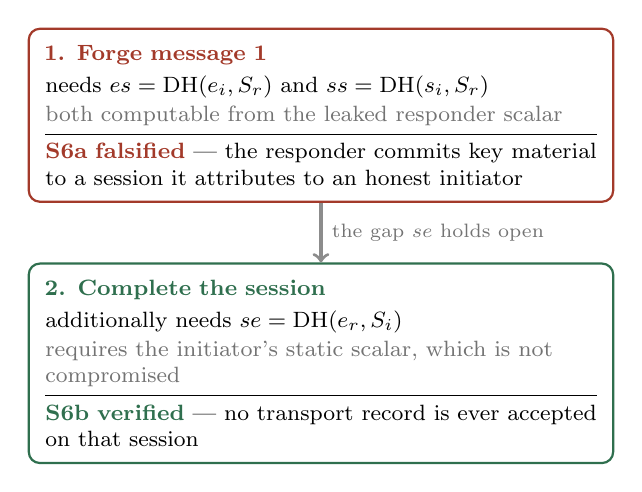
\begin{tikzpicture}[x=1cm,y=1cm,font=\footnotesize]
  \node[draw=badred,thick,rounded corners,align=left,inner sep=6pt,
        text width=7.0cm] (a) at (0,0)
    {\textbf{\color{badred}1. Forge message 1}\\[2pt]
     needs $es=\mathrm{DH}(e_i,S_r)$ and $ss=\mathrm{DH}(s_i,S_r)$\\[1pt]
     {\color{black!55}both computable from the leaked responder scalar}\\[3pt]
     \hrule\vspace{3pt}
     {\color{badred}\textbf{S6a falsified}} --- the responder commits key
     material to a session it attributes to an honest initiator};
  \node[draw=okgreen,thick,rounded corners,align=left,inner sep=6pt,
        text width=7.0cm] (b) at (0,-3.15)
    {\textbf{\color{okgreen}2. Complete the session}\\[2pt]
     additionally needs $se=\mathrm{DH}(e_r,S_i)$\\[1pt]
     {\color{black!55}requires the initiator's static scalar, which is not
      compromised}\\[3pt]
     \hrule\vspace{3pt}
     {\color{okgreen}\textbf{S6b verified}} --- no transport record is ever
     accepted on that session};
  \draw[->,very thick,black!45] (a.south) -- node[right,black!55,align=left]
    {\scriptsize the gap $se$ holds open} (b.north);
\end{tikzpicture}
}
\caption{With the responder's static key compromised, two adjacent
authentication levels separate. The static-ephemeral term \(se\) is the whole
of the difference, and the property lives in the gap between them.}
\label{fig:kci}
\end{figure}

Key-compromise impersonation asks whether compromising a party's own long-term
key lets an attacker impersonate \emph{others} to it. We asked it at two
levels, and the levels separate (Figure~\ref{fig:kci}).

\para{The responder does commit.} Producing a well-formed message~1 in the
name of an honest initiator requires \(es=\mathrm{DH}(e_i,S_r)\) and
\(ss=\mathrm{DH}(s_i,S_r)\). Both are computable from the leaked responder
scalar, so an attacker can drive the responder to commit transport keys for a
session it attributes to that initiator. Tamarin refutes the
commitment-level lemma (S6a) and returns the trace.

\para{The responder never completes.} Deriving those transport keys
additionally requires \(se=\mathrm{DH}(e_r,S_i)\), and that needs either the
responder's ephemeral scalar or the initiator's static scalar. The attacker
has neither. Tamarin verifies the completion-level lemma (S6b): the responder
never accepts a transport record on such a session.

\para{Why the distinction is operational.} WireGuard's KCI resistance depends
on treating a session as established only once authenticated traffic has
arrived, not once the handshake response has been sent. A model with a single
``session established'' event would report one verdict where there are two,
and would locate the property in the wrong place.

\subsection{KEM-derived pre-shared keys}

If the pre-shared key is to come from a KEM rather than from manual
configuration---the construction Rosenpass~\cite{rosenpass2023} uses---the
question is what that KEM must bind. We modelled two: one whose shared secret
depends on the encapsulation key, and one whose shared secret depends only on
the encapsulation randomness, together with the re-encapsulation capability
that absence of binding confers.

\para{Binding is the whole of it.} With binding, secrecy of the established
pre-shared key is proved (P12a). Without it, the attacker redirects an
observed ciphertext to an encapsulation key of its own and recovers the
pre-shared key outright (P12b). The failure is not a weakness in any
primitive: confidentiality and integrity of the KEM are untouched, and only
the binding is missing. In the vocabulary of Cremers, Dax and
Medinger~\cite{cremers2024kembinding} the separating property is
MAL-BIND-K-PK, which ML-KEM satisfies.

\para{One query we could not settle.} A third query, asking whether the
responder's view of the established key is sound, returned inconclusive
(P12c): a bare encapsulation authenticates nobody, and the honest statement is
disjunctive in a way ProVerif's approximation could not decide. We report it
as inconclusive rather than restate it until it passed. An undecided query is
a result; a restated one is not.

\section{The Cost of Post-Quantum Migration}
\label{sec:pq}

The analysis in this section requires no computation and no measurement. Every
figure follows arithmetically from the wire-format layout of
Section~\ref{sec:modelling} and the published parameter sizes of
ML-KEM~\cite{fips203}. That makes it the most robust part of the paper: it
does not depend on the machine it was produced on, and it cannot be disturbed
by a prover's resource limits.

\subsection{Packet growth}

\begin{table}[t]
\centering
\caption{In-band KEM substitution, sizes in bytes. The substitution modelled
is the cheapest one possible, so these are a lower bound on any in-band
design.}
\label{tab:pqsizes}
\footnotesize
\begin{tabular}{@{}lrrrr@{}}
\toprule
KEM & $ek$ & $ct$ & initiation & response \\
\midrule
X25519 (baseline) & 32 & 32 & 148 & 92 \\
\midrule
ML-KEM-512 & 800 & 768 & 916 ($\times$6.2) & 828 ($\times$9.0) \\
ML-KEM-768 & 1184 & 1088 & 1300 ($\times$8.8) & 1148 ($\times$12.5) \\
ML-KEM-1024 & 1568 & 1568 & 1684 ($\times$11.4) & 1628 ($\times$17.7) \\
\bottomrule
\end{tabular}

\end{table}

We model the cheapest possible in-band substitution: the initiator's 32-byte
ephemeral public value becomes an encapsulation key, the responder's becomes
the corresponding ciphertext, and every other field keeps its length. Because
this is the minimal construction, the resulting sizes
(Table~\ref{tab:pqsizes}) are a \emph{lower bound} on any in-band design,
which is what makes the conclusion below robust rather than contingent on a
particular protocol sketch. An initiation grows by a factor of \wgKemGrowth{}
at ML-KEM-768 and \wgKemTenGrowth{} at ML-KEM-1024.

\subsection{Path reachability}

\begin{figure}[t]
\centering
\resizebox{\columnwidth}{!}{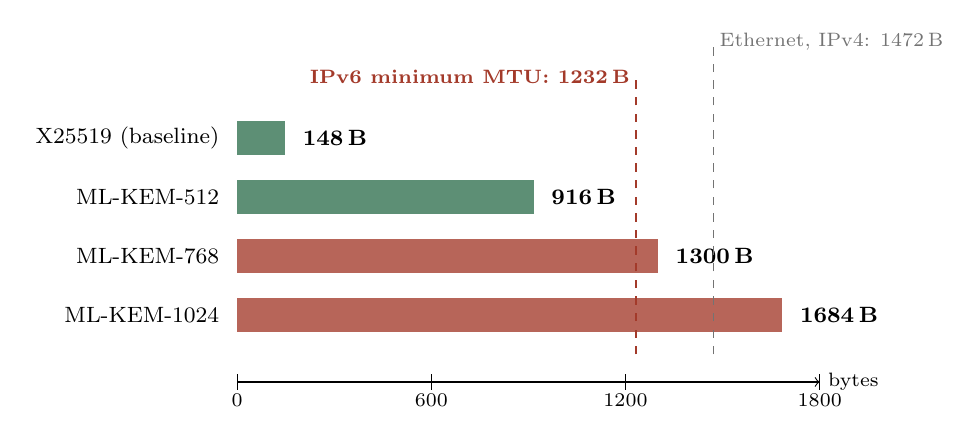
\begin{tikzpicture}[x=1cm,y=1cm]
  \footnotesize
  \fill[okgreen!78] (0,-0.22) rectangle (0.608,0.22);
  \node[anchor=east] at (-0.12,-0.0) {X25519 (baseline)};
  \node[anchor=west] at (0.728,-0.0) {\bfseries 148\,B};
  \fill[okgreen!78] (0,-0.97) rectangle (3.766,-0.53);
  \node[anchor=east] at (-0.12,-0.75) {ML-KEM-512};
  \node[anchor=west] at (3.886,-0.75) {\bfseries 916\,B};
  \fill[badred!78] (0,-1.72) rectangle (5.344,-1.28);
  \node[anchor=east] at (-0.12,-1.5) {ML-KEM-768};
  \node[anchor=west] at (5.464,-1.5) {\bfseries 1300\,B};
  \fill[badred!78] (0,-2.47) rectangle (6.923,-2.03);
  \node[anchor=east] at (-0.12,-2.25) {ML-KEM-1024};
  \node[anchor=west] at (7.043,-2.25) {\bfseries 1684\,B};
  \draw[badred,dashed,thick] (5.065,-2.75) -- (5.065,0.78);
  \node[badred,anchor=east,inner sep=2pt,font=\scriptsize,font=\scriptsize\bfseries] at (5.065,0.78) {IPv6 minimum MTU: 1232\,B};
  \draw[black!55,dashed,thin] (6.052,-2.75) -- (6.052,1.22);
  \node[black!55,anchor=west,inner sep=2pt,font=\scriptsize] at (6.052,1.22) {Ethernet, IPv4: 1472\,B};
  \draw[->] (0,-3.1) -- (7.400,-3.1) node[anchor=west] {\scriptsize bytes};
  \draw (0.000,-3.2) -- (0.000,-3.0) node[anchor=north,yshift=-4pt] {\scriptsize 0};
  \draw (2.467,-3.2) -- (2.467,-3.0) node[anchor=north,yshift=-4pt] {\scriptsize 600};
  \draw (4.933,-3.2) -- (4.933,-3.0) node[anchor=north,yshift=-4pt] {\scriptsize 1200};
  \draw (7.400,-3.2) -- (7.400,-3.0) node[anchor=north,yshift=-4pt] {\scriptsize 1800};
\end{tikzpicture}
}
\caption{Initiation size against the usable UDP payload of each path. The
ML-KEM-768 bar crosses the IPv6 minimum-MTU rule; that crossing is the whole
of the argument in this section.}
\label{fig:mtu}
\end{figure}

\begin{table}[t]
\centering
\caption{ML-KEM-768 initiation against \wgPaths{} representative path MTUs.
Only the first row is a guarantee; the others are common cases.}
\label{tab:pqmtu}
\footnotesize
\begin{tabular}{@{}lrrr@{}}
\toprule
Path & MTU & usable UDP & ML-KEM-768 initiation \\
\midrule
IPv6 minimum MTU & 1280 & 1232 & \textbf{exceeds by 68\,B} \\
Ethernet, IPv4 & 1500 & 1472 & fits, 172\,B spare \\
Ethernet, IPv6 & 1500 & 1452 & fits, 152\,B spare \\
PPPoE, IPv4 & 1492 & 1464 & fits, 164\,B spare \\
Tunnel stacking, IPv4 & 1400 & 1372 & fits, 72\,B spare \\
\bottomrule
\end{tabular}

\end{table}

RFC~8200~\cite{rfc8200} requires every IPv6 link to carry a
\wgIpvsixMtu-byte datagram. After an IPv6 header of 40\,B and a UDP header of
8\,B, the usable payload is \wgIpvsixPayload\,B. An in-band ML-KEM-768
initiation is \wgKemInit\,B. It exceeds that payload by \wgOvershoot\,B, and a
datagram that does not fit the IPv6 minimum MTU has no guaranteed path
(Figure~\ref{fig:mtu}, Table~\ref{tab:pqmtu}). Path MTU discovery for datagram
transports~\cite{rfc8899} can find a larger path when one exists, but it
cannot manufacture one where it does not.

\para{The chain, stated plainly.} Each link below is individually
unremarkable, and the conclusion is not:

\begin{quote}
KEM parameter sizes \(\rightarrow\) datagram size \(\rightarrow\) path MTU
\(\rightarrow\) fragmentation or PMTUD failure \(\rightarrow\) the handshake
is unreachable on some paths \(\rightarrow\) the architecture must change.
\end{quote}

This is why post-quantum designs for WireGuard either restructure the
handshake around KEMs from the start~\cite{hulsing2021pqwireguard} or perform
the key agreement over a separate channel and inject the result into the
pre-shared key slot. Rosenpass~\cite{rosenpass2023} takes the second route,
and the analysis above supplies the reason it is necessary rather than merely
convenient.

\para{What migration costs beyond bytes.} There is a real tension worth
naming. WireGuard's single-packet, stateless handshake is itself an
engineering asset: it needs no fragment reassembly, holds no state before
authentication, and is what makes the cookie mechanism possible. Post-quantum
migration threatens precisely that asset. ML-KEM-512 would fit every path
considered at \wgKemFiveInit\,B, but at a security level most deployments will
not choose; ML-KEM-1024, at \wgKemTenInit\,B, fits none of them.

\subsection{Three dimensions, one conclusion}

Combining this section with Section~\ref{sec:results}:

\begin{itemize}\itemsep2pt
\item \emph{Packet size.} An in-band initiation grows by a factor of
      \wgKemGrowth{} at ML-KEM-768 and \wgKemTenGrowth{} at ML-KEM-1024.
\item \emph{Path reachability.} Above ML-KEM-512, in-band substitution loses
      the guarantee of a usable path.
\item \emph{Assumption strength.} A KEM-derived pre-shared key preserves the
      properties of a configured one only if the KEM binds its shared secret
      to the encapsulation key; without that binding the pre-shared key is
      recoverable while every primitive remains unbroken (P12a/P12b).
\end{itemize}

The cost of post-quantum migration is not merely computational. It appears
along all three dimensions at once, and a design that addresses only one of
them has not addressed the problem.

\section{Prover Comparison and Limitations}
\label{sec:discussion}

Because the protocol was transcribed once and handed to both provers, the
differences reported here are attributable to the provers.
Table~\ref{tab:provers} aggregates the result matrix by tool.

\begin{table}[t]
\centering
\caption{The two provers on one transcription. ``Wall-clock spent undecided''
is budget consumed without producing a verdict; it is a cost, not a result.}
\label{tab:provers}
\footnotesize
\begin{tabular}{@{}lrr@{}}
\toprule
 & ProVerif & Tamarin~1.12.0 \\
\midrule
Properties posed & 12 & 6 \\
Proved & 6 & 5 \\
Attack found & 2 & 1 \\
Inconclusive & 1 & 0 \\
Non-terminating & 3 & 0 \\
\midrule
Wall-clock to a verdict (s) & \textit{n/r} & \textit{n/r} \\
Wall-clock spent undecided (s) & --- & --- \\
\bottomrule
\end{tabular}

\end{table}

\ifwgtimings
\begin{figure}[t]
\centering
\resizebox{\columnwidth}{!}{%% no per-query timings in results/results.json; figure omitted
}
\caption{Wall-clock cost of every property, grouped by prover. The bars
marked \(\dagger\) reached the budget without reaching a verdict; two of the
three are the properties Tamarin settles in the group below.}
\label{fig:cost}
\end{figure}
\fi

\subsection{Where the transcriptions diverge}

Two differences were unavoidable, and both are consequences of how the provers
handle Diffie-Hellman.

\para{Term construction.} ProVerif required the two-symbol
\(\mathit{pk}/\mathit{dh}\) encoding of Section~\ref{sec:modelling} to bound
term depth. Tamarin normalises Diffie-Hellman terms natively and uses its
built-in theory directly. The two formulations agree on the equational theory;
they differ in what the attacker can syntactically construct, and only one of
the provers needs the restriction.

\para{Expressing compromise.} Compromise is expressed with ProVerif's phase
mechanism and with action facts in Tamarin. Phases impose a global ordering,
which is exactly what harvest-now-decrypt-later needs and is why the
post-quantum experiment lives on the ProVerif side. Action facts let a lemma
quantify over the relative order of individual compromise and session events,
which is what the KCI lemmas need.

\subsection{The resource profile, and what it is evidence for}

The contrast is sharp and one-directional.
\ifwgtimings
ProVerif proved what it could prove quickly---\wgPvSpan\,s across the
properties it decided---and failed completely on the rest, exhausting the
budget rather than slowing down. Tamarin decided every lemma we posed it,
including both KCI levels, in \wgTamSpan\,s and \wgTamSteps{}
constraint-solving steps (Figure~\ref{fig:cost}).
\else
ProVerif proved what it could prove well inside the budget and failed
completely on the rest, exhausting the budget rather than slowing down.
Tamarin decided every lemma we posed it, including both KCI levels, in
\wgTamSteps{} constraint-solving steps. Per-query wall-clock cost is recorded
per run in \texttt{results/results.json} and reproduced in
\texttt{docs/generated/cost.md}.
\fi

\para{An identifiable cause.} The \wgPvNonterm{} ProVerif properties left
undecided are agreement in the responder-to-initiator direction and both KCI
levels. The KCI failures have a diagnosis. Releasing the responder's static
scalar unlocks every responder-side Diffie-Hellman term for the attacker, and
the resulting clause set diverges; bounding the initiator to a single session
reduced memory pressure but not the divergence. Tamarin's constraint solving
is not sensitive in the same way, because it reasons backwards from the
property rather than saturating forwards from the rules.

\para{A practical rule.} The division of labour that emerged is not the
textbook one, and it is worth stating in the form this project actually found
it. Reach for ProVerif when the property is secrecy or a correspondence over
honest parties, when many variants of one model must be run, or when a global
staging of attacker capability---such as a quantum transition---is the natural
formulation; it is fast and fully automatic in that regime. Reach for Tamarin
when a long-term secret is compromised as part of the scenario rather than
after it, when the property depends on the relative ordering of specific
events, or when explicit mutable state is required. The KCI pair of
Section~\ref{sec:results} is all three at once, and it is the single clearest
instance in this work.

\para{What this is not.} This is a resource observation from one protocol, not
a general claim about the tools. It is recorded because comparisons of this
kind are rarely published with the failures included, and the failures are the
informative part.

\subsection{Limitations}

\para{The symbolic abstraction.} Both models assume a Dolev-Yao attacker and
perfect primitives. They say nothing about side channels, implementation
defects, or concrete security parameters. The Diffie-Hellman abstraction
treats every 32-byte value as \(g^t\) for some \(t\), which excludes
small-subgroup and invalid-curve behaviour and the all-zero output check.

\para{The transcript hash.} Modelling \(h\) after step \(i\) as a flat
collision-resistant function of the prefix binds the same data as the iterated
formulation, but it assumes the hash chain is collision-free as a whole rather
than deriving that from the properties of a single compression function. A
collision attack on BLAKE2s would be invisible to this model, as it would be
to any symbolic one.

\para{Non-terminating queries prove nothing.} Of \wgProps{} properties,
\wgNonterm{} were left undecided. A non-terminating query is not a proof of absence: it says the prover
could not settle the question within the budget, and nothing about the
protocol. Two of the three were subsequently decided by Tamarin; the third,
agreement in the responder-to-initiator direction, remains open in this
artifact. The KCI queries were additionally attempted on the ProVerif side
with the initiator bounded to one and two sessions; those runs would have
established the property for that number of sessions only, and are reported as
non-terminating in any case.

\para{Verification, not measurement.} This artifact verifies the handshake. It
does not measure it. The network laboratory accompanying the repository---a
multi-node network namespace topology with traffic capture and injected
wide-area conditions---is provided as a Linux companion and was not exercised
for this release, because network namespaces are a Linux kernel interface with
no macOS equivalent and the development machine is an Apple Silicon laptop. No
latency or throughput figure appears anywhere in this paper, and none should
be inferred from it. Section~\ref{sec:pq} depends on no measurement
whatsoever.

\para{Attribution.} Where the conclusions here differ from prior work
\cite{donenfeld2018formal,lipp2019cryptoverif}, the difference is a modelling
assumption rather than a finding, and the assumptions are stated in
Section~\ref{sec:modelling} so that such differences can be traced.

\section{Conclusion}

Transcribing the WireGuard handshake once and giving it to two provers
produced three findings a single-tool analysis would not have, and one
property of the artifact itself.

\para{The pre-shared key's contribution became an experiment.} Two models
differing in one line, one proved and one refuted against an attacker holding
a discrete-logarithm oracle. What was previously an assertion about
\texttt{IKpsk2} is now a control with a recorded verdict on each arm
(Table~\ref{tab:psk}).

\para{KCI resistance turned out to have a location.} It is not a property of
the handshake as a whole but of the interval between committing transport keys
and accepting traffic, and the static-ephemeral term \(se\) is what holds that
interval open. Finding this required asking the question at two levels, and
answering it required the prover that ProVerif's saturation had defeated.

\para{Post-quantum cost is not one number.} Following KEM parameter sizes
through to path MTU shows an in-band ML-KEM-768 handshake exceeding the IPv6
minimum by \wgOvershoot\,B. The cost appears as packet size, path
reachability, and assumption strength simultaneously, and a design that
addresses one of the three has not addressed the problem.

\para{The disagreements are the informative part.} The \wgNonterm{}
properties nobody could decide sit in Table~\ref{tab:results} alongside the
rest. A
result matrix in which every cell is green says less about a pair of provers
than one in which the disagreements are visible. That this remains true of
every future run is not a promise but a build step: the tables, figures and
quoted numbers in this paper are regenerated from the provers' own output
each time the document is compiled.


\bibliographystyle{IEEEtran}
\bibliography{refs}

\end{document}
